\chapteruaf{Using Page Allocation Timings to Detect VMI}\label{MMapChap}

\section{Motivation}\label{MMapChap-Intro}
In this chapter we discuss a simple statistical analysis of the time taken to map a page in main memory. When we look at resources shared between the Host and the Guest one of the most obvious ones is main memory. In the x86-64 processor main memory by the Memory Management Unit (MMU), which uses a process called paging to control which data and instructions are held in main memory. 

When a VMI program is used on a guest memory is mapped from the memory space of the guest to the memory space of the host (which, for brevity, we will refer to as guest-space and host-space respectively). We believe this mapping from guest-space to host-space will affect which pages are in memory to a degree that is measurable in the time required to map a page in memory.  


\section{Experimental Design}\label{MMapChap-ExpDesign}

For our initial experiment we aim to determine whether or not a guest VM can detect that it is being monitored by a VMI process. We begin by using the same experimental hardware described in chapter 2.  For our experimental setup we use a KVM and a Xen host. Each host runs a single VM of Ubuntu 14.04 as described in chapter II.  

On the host the VMI agent was run continuously. We did three trials: one where the process-list command was run, one where the module-list command was run, and one where the map-addr command was run. In each case the VMI program is continually run on the guest VM. 


On the guest side a probe is set up. This probe uses the C++11 chrono object~\cite{_chrono_2014} which gives us nanosecond resolution. For each iteration the time stamp is recorded, a page is mapped and unmapped from memory using the mmap function~\cite{_mmap2_2014}, and then the timestamp is again recorded. The difference between the second time stamp and the first time stamp are taken and this result is recorded as the time taken to map and unmap a page. As mentioned earlier however a small correction is made and the overhead time in the previous section is subtracted from the result to give our final result.  A control sample where no VMI agent is being run on the guest is also taken. 


\begin{enumerate}\label{MMapAlg}
	\item Mark Timestamp $t_0$
	\item map page in memory
	\item unmap page in memory
	\item Mark Timestamp $t_1$
	\item Record $t_1$-$t_0$
\end{enumerate}

\section{Results and Analysis}\label{MMapChap-Results}

The first step of our analysis is to compare the histograms of the control data with data here VMI is used.  It can be seen immediately (figs ~\ref{XenMMapHist1} and ~\ref{KVMMMapHist1}) that not only are the samples with VMI different from the control sample but they are also different f
rom each other as well. One should note that these histograms are zoomed in to give a better insight into the data. There are still small pockets of data after the 10,000ms bin but these are so small as to be not evident in the histograms.  The next step is to determine whether or not these datasets are statistically different from the data in the control sample. To do this we use two statistical tests, which determine whether or not two populations share the same mean. The first is Welch's t-test ~\cite{welch_generalization_1947} which determines whether the mean of two populations is the same. The second is the Mann Whitney U-test which again measures whether the two means of the population are the same.


	\begin{figure}[p!]\label{XenMMapHist1}
	  \centering
	  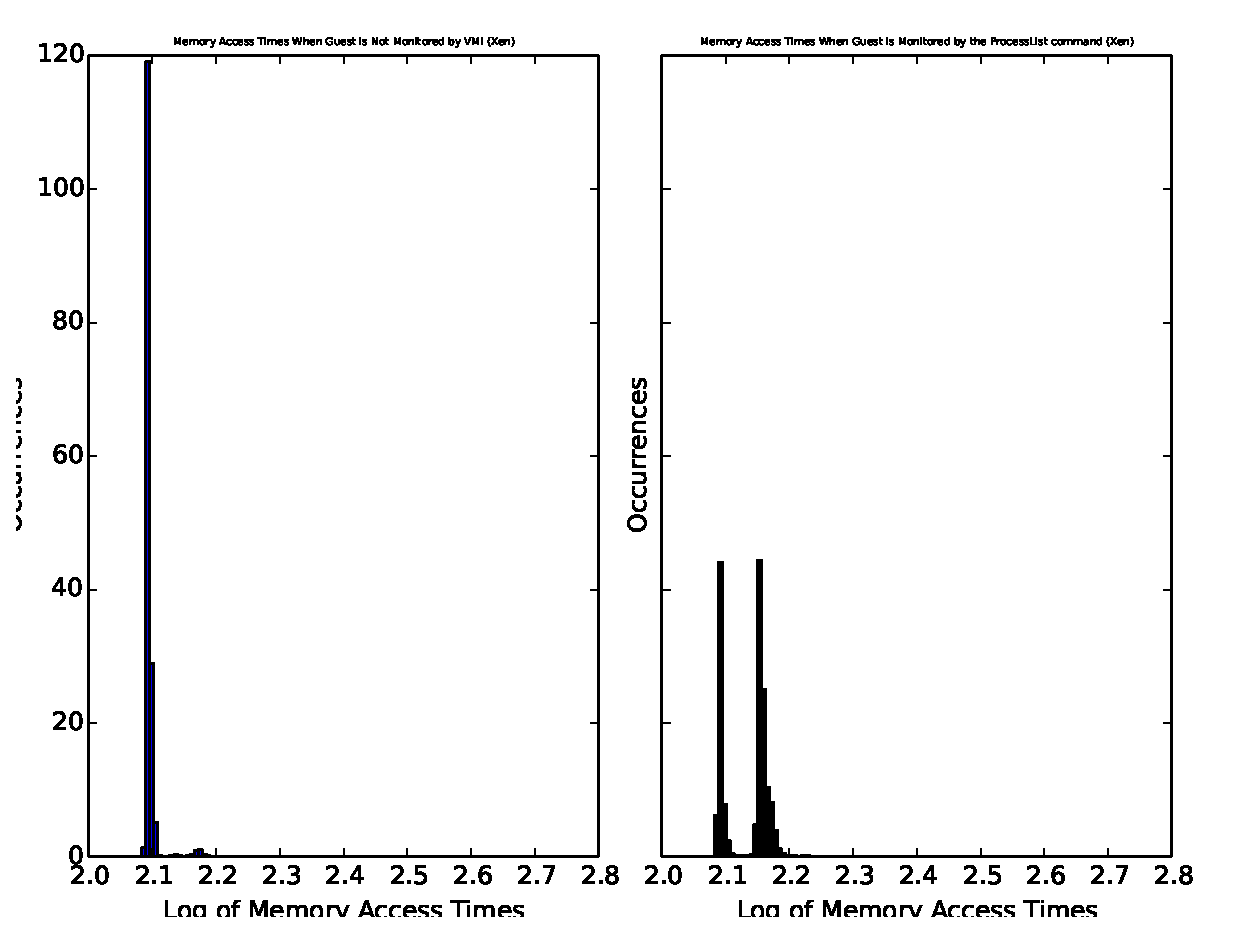
\includegraphics[width=\textwidth]{figures/XenNoVMIVsProcList.eps}
	  \caption{Histograms of the log of mmap time when a Xen VM is not observed by VMI (left) and observed by the process-list command (right)}
	\end{figure}


	\begin{figure}[p!]\label{KVMMMapHist1}
	  \centering
	  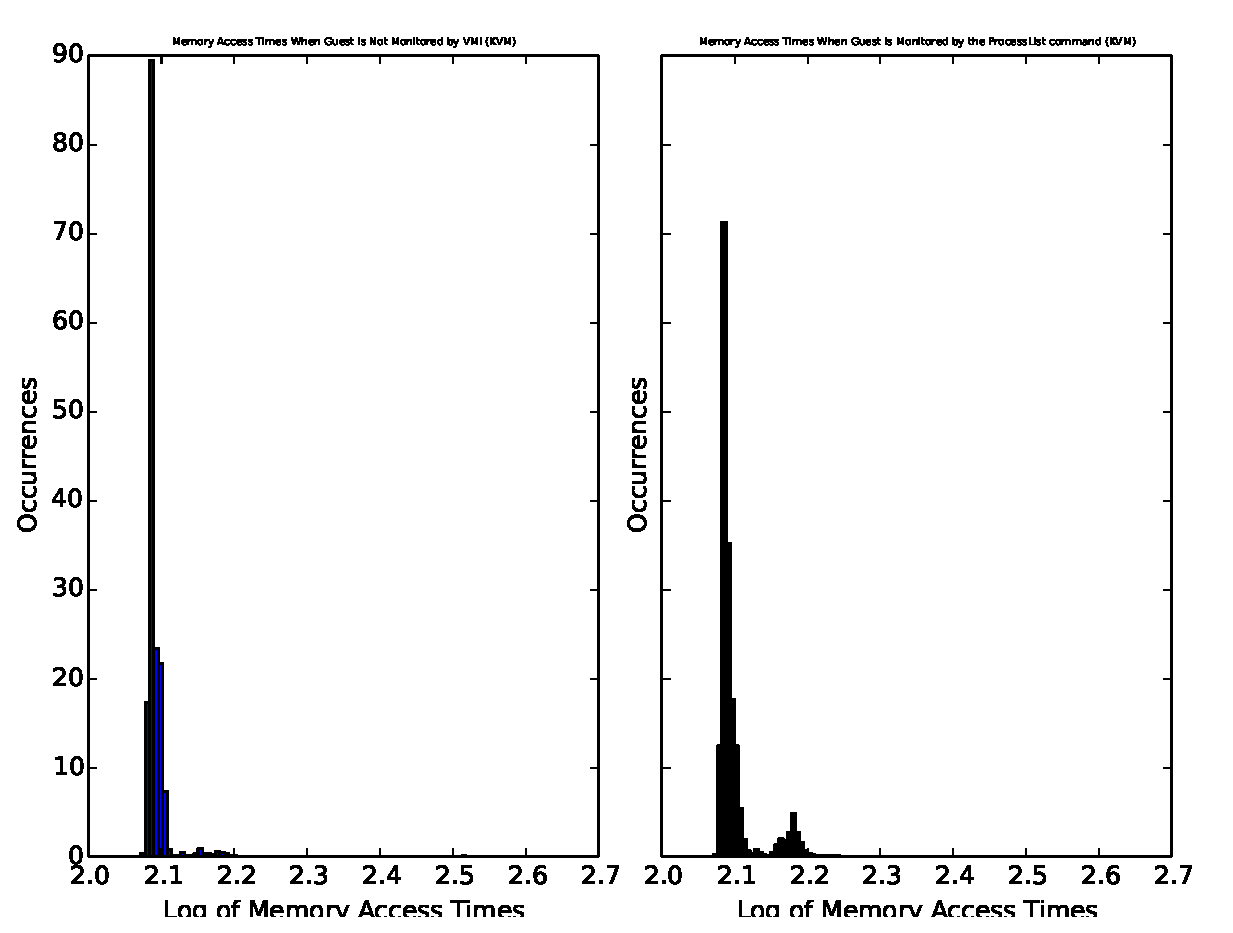
\includegraphics[width=\textwidth]{figures/KVMMMApTestNoVMIvsProcList.eps}
	  \caption{Histograms of the log of mmap time when a KVM VM is not observed by VMI (left) and observed by the process-list command (right)}
	\end{figure}

In both cases we begin with the null hypothesis that the mean of a sample not being monitored by VMI is the same as the mean of a sample which was being monitored by some form of VMI. The results of these tests are shown in table ~\ref{TStatsMMap1}. 
As we can see the results of the likelihood of the means of the two populations being is extremely low. It should be noted here that while all of the p-values are 0 this is strictly speaking not possible for finite populations. Instead this is a limitation of IEEE floating point arithmetic and a value of 0 should be taken as a value of less than $10^{-6}$.

	\begin{table}[p!]
		\centering
		\begin{tabular}{| c | c | c | c |}
			\hline
			Hypervisor & mapPage & modList & procList  \\ \hline
			Xen & -4361 & -5678 & -1691  \\  \hline
			KVM & -903 & -1000 & -632  \\ \hline
		\end{tabular}
		\label{TStatsMMap1}
		\caption{T stats for Xen and KVM compared to the null hypothesis that no VMI is being used}
	\end{table}

	\begin{table}[p!]
		\centering
		\begin{tabular}{| c | c | c | c |}
			\hline
			Hypervisor & mapPage & modList & procList  \\ \hline
			Xen & $3.73x10^{8}$ & $8.71x10^{8}$ & $7.43x10^{8}$  \\  \hline
			KVM & $8.34x10^{8}$ & $1.02x10^{9}$ & $3.26x10^{8}$ \\  \hline
		\end{tabular}
		\label{MannWhitneyMMap1}
		\caption{U stats for Xen and KVM compared to the null hypothesis that no VMI is being used}
	\end{table}



The next question to arise is this are these patterns unique to VMI or can theya be reproduced by other means? To answer this we first consider which factors can impact time taken to map a page are page faults and cache misses~\cite{bryant_computer_2003}.  At the scale of time being dealt with in this experiment cache misses will likely not be a significant factor given that they tend to operate in the 100ns range. As a result we will instead focus on page faults. 

\section{Elimination Experiments}

For this portion of the experiment we will test whether a VM with more memory will cause similar patterns in the time it takes to map a page  to those caused when a VM is being monitored by a VMI agent. We begin this portion of the experiment by cloning our initial VM but changing configuration so the VM has 4GB of RAM instead of the one it had earlier. The probe process as described in section ~\ref{MMapChap-ExpDesign} is repeated. The results are compared to the null hypothesis that the target VM is being monitored by the process-list program. 


We can see that these histograms are distinctly different (fig ~\cite{KVMMMapVS4Gig}. We then compare the two samples using the Mann-Whitney U test and the t-test we can see that the p-values are well outside our critical range and thus we reject the null hypothesis that two samples are the same. 

	\begin{figure}[p!]\label{KVMMMapVS4Gig}
	  \centering
	  \includegraphics[width=\textwidth]{figures/ProcListVS4GigKVM.eps}
	  \caption{Histograms of the log of mmap time when a KVM VM observed by the process-list command(left) and when a KVM VM has 4GB of RAM (right)} 
	\end{figure}

Next we test whether a VM which has more VCPUs can be confused with the signal of a VMI agent. We begin this portion of the experiment by cloning our initial VM but changing configuration so the VM has 3 VCPUs  instead of the one it had earlier. The probe process described in ~\ref{MMapChap-ExpDesign} is repeated. We again make the null hypothesis that the target VM is being monitored by the process-list program. 

We can see that these histograms are distinctly different (fig ~\ref{KVMMMapVS43VCPU}). We then compare the two samples using the Mann-Whitney U test and the t-test we can see that the p-values are well outside our critical range and thus we reject the null hypothesis that two samples are the same.


	\begin{figure}[p!]\label{KVMMMapVS43VCPU}
	  \centering
	  \includegraphics[width=\textwidth]{figures/ProcListVS3CPUKVM.eps}
	  \caption{Histograms of the log of mmap time when a KVM VM observed by the process-list command(left) and when a KVM VM has 3VCPUs (right)}
	\end{figure}


	\begin{table}[p!]\label{TableCPURAM}
		\centering
		\begin{tabular}{| c | c | c |}
			\hline
			 ``fill something in here '' & Mann-Whitney  & t-test  \\ \hline
			3VCPU & $ 1.184x10^{7}$ & $174.0$  \\  \hline
			4GB RAM & $1.373x10^{7} $ & $147.1$   \\  \hline
		\end{tabular}
		\label{MultiCPUsAndRam}
		\caption{U stat and t stat for populations taken when the VM had 4GB of RAM or 3VCPUs compared to the null hypothesis that they were being monitored by a VMI agent.}
	\end{table}

We next attempt to determine whether or not the number of VMs running on the same host will produce a signal similar to the one produced by a VM being monitored by a VMI agent. We begin our experiment by making three identical clones of our initial VM (now called VM-A) which will be labeled VM-B, VM-C, and VM-D as shown in figure ~\ref{Fig4VMTest}. We run an experiment initially where only VMs A and B are running. The probe described in section ~\ref{MMapChap-ExpDesign} was run on VM-A while VM-B was idle. We repeat this process with VMs A-C running and again with VMs A-D running.  We then compare each of these samples taken to the samples when a VM is being monitored by VMI (insert fig). 
	
	\begin{figure}[p!]\label{Fig4VMTest}
	  \centering
	  \includegraphics[width=\textwidth]{figures/BM_graph2_cropped.png}
	  \caption{Diagram of multi VM experiment} 
	\end{figure}


An interesting phenomenon occurs when one looks at the means of each of the samples taken in this experiment. When we compare the sample taken with two VMs running to our control sample there is a substantial decrease in the mean time taken to map a page. This average time then increases when a third and fourth VM are added (fig ~\ref{Fig4VMTest}).

	\begin{figure}[p!]\label{Fig4VMTestCentOS}
		\centering
		\includegraphics[width=\textwidth]{figures/mmapTimesOverVMsIdentical.png}
		\caption{Average MMap vs How many VMs are present}
	\end{figure}

What is causing this decrease in average mmap timing? We hypothesize that since the VMs are clones of each other the time merging of identical memory among the VMs has decreased the average memory access time by decreasing the number of cache misses since kernel data strutures are more likely to be in cache when accessed by another VM with an identical kernel. To test this hypothesis we repeat this exeriment however instead of cloning VM-A for VMs B-D we use CentOS Linux. If our hypothesis is correct we will now see a decrease in the average time taken to map a page when VM-C is added. We can see this occurred in fig ~\ref{Fig4VMTestCentOS} Thus indicating that our hypothesis was correct.

\begin{figure}[p!]\label{Fig4VMTestCentOS}
		\centering
		\includegraphics[width=\textwidth]{figures/CentOSTimesVsVMKVMANDXEN.png}
		\caption{Average MMap vs How many VMs are present when VMs B-D are CentOS VMs}
	\end{figure}

 

\section{Conclusion}
In this chapter we successfully introduced a method for detecting VMI as well as distinguishing between which VMI agent was used. It was also distinguish between multiple VMs being used as well as different levels of resource allocation. While it is impossible to exhaustively test all scenarios we consider this experiment to be a success as it did detect VMI. However it was not without its limitations. The VMI agent had to be run continuously without break on the VM in order for this method to be successful. This means that while successful in a technical sense it isn't especially realistic. 